% Created 2024-04-22 Δευ 12:13
% Intended LaTeX compiler: pdflatex
\documentclass[11pt]{article}
\usepackage[utf8]{inputenc}
\usepackage[T1]{fontenc}
\usepackage{graphicx}
\usepackage{longtable}
\usepackage{wrapfig}
\usepackage{rotating}
\usepackage[normalem]{ulem}
\usepackage{amsmath}
\usepackage{amssymb}
\usepackage{capt-of}
\usepackage{hyperref}
\usepackage{booktabs}
\usepackage{import}
\usepackage[LGR, T1]{fontenc}
\usepackage[greek, english, american]{babel}
\usepackage{alphabeta}
\usepackage{esint}
\usepackage{mathtools}
\usepackage{esdiff}
\usepackage{makeidx}
\usepackage{glossaries}
\usepackage{newfloat}
\usepackage{minted}
\usepackage{chemfig}
\usepackage{svg}
\author{Vidianos Giannitsis}
\date{\today}
\title{Εισαγωγή - Στατιστικά Στοιχεία}
\hypersetup{
 pdfauthor={Vidianos Giannitsis},
 pdftitle={Εισαγωγή - Στατιστικά Στοιχεία},
 pdfkeywords={},
 pdfsubject={},
 pdfcreator={Emacs 29.3 (Org mode 9.6.15)}, 
 pdflang={English}}
\makeatletter
\newcommand{\citeprocitem}[2]{\hyper@linkstart{cite}{citeproc_bib_item_#1}#2\hyper@linkend}
\makeatother

\usepackage[notquote]{hanging}
\begin{document}

\maketitle
\tableofcontents


\section{Εισαγωγή}
\label{sec:org1f77ea1}
Τα υπολείμματα τροφών αποτελούν μία από τις σημαντικότερες κατηγορίες οργανικών αποβλήτων. Ο οργανισμός τροφίμων και αγρονομίας των ηνωμένων πολιτείων (FAO) υπολογίζει πως περίπου το 1/3 της παγκόσμιας παραγωγής τροφών (περίπου 1.3 δις τόνοι ετησίως) χάνεται κατά την παραγωγική διαδικασία ή απορρίπτεται. Κάποιες από αυτές τις απώλειες είναι αναπόφευχτες, αλλά πολλές θα μπορούσαν να αποφευχθούν ή τα υπολείμματα να συλλεχθούν για μία καλύτερη αξιοποίηση, καθώς οι κλασσικές τεχνικές, όπως η υγειονομική ταφή ή η αποτέφρωση, δημιουργούν προβλήματα όπως οι ανεξέλεγκτες εκπομπές μεγάλων ποσοτήτων αερίων του θερμοκηπίου (Wu et al. 2022; Zhang et al. 2020; Ishangulyyev, Kim, and Lee 2019).

Συγκεκριμένα, έχει προσδιοριστεί πως το ισοδύναμο διοξειδίου του άνθρακα που παράγεται λόγω της μη ορθής αυτής διαχείρισης των υπολείμματων ανέρχεται στους 3.3 δις τόνους (Taheri et al. 2021) . Ακόμη, έχει βρεθεί πως τα υπολείμματα τροφών που οφείλονται μόνο στην απόρριψη τροφών από καταναλωτές σε ανεπτυγμένες χώρες είναι σχεδόν όσα παράγουν οι υπό σακχάριες και αφρικανικές χώρες συνολικά (περίπου 230 εκατομμύρια). Οπότε η αποφυγή της δημιουργίας τόσων υπολειμμάτων - ή η καλύτερη αξιοποίηση τους - θα μπορούσε να λύσει πολλά προβλήματα υποσιτισμού. Ακόμη και στον οικονομικό τομέα, δημιουργούνται σοβαρά προβλήματα από την ανεξέλεγκτη αυτή απόρριψη καθώς η καθαρή αξία των τροφών που χάνονται ή απορρίπτονται σε κάποιο σημείο της εφοδιαστικής αλυσίδας είναι 936 δις δολλάρια ανά έτος με ελάχιστο κέρδος, καθώς πολύ μικρές ποσότητες των υπολειμμάτων αυτών αξιοποιούνται (Ishangulyyev, Kim, and Lee 2019) . Συμπερασματικά, η δημιουργία αυτών των υπέρογκων ποσοτήτων υπολειμμάτων τροφών πλήγει κάθε πυλώνα της βιωσιμότητας και είναι ένα πάρα πολύ σοβαρό πρόβλημα.

Μία από τις βασικότερες υποκατηγορίες υπολειμμάτων τροφών είναι τα οικιακά υπολείμματα τροφών. Αποτελούν το μεγαλύτερο κομμάτι της παγκόσμιας παραγωγής υπολειμμάτων τροφών, αποτελώντας περίπου το \(61 \%\) αυτής (“Statista - The Statistics Portal” n.d.) . Στο \figurename\textasciitilde{} \ref{fig:orge19f8e8} φαίνεται η παγκόσμια παραγωγή υπολειμμάτων τροφών ανά τομέα.
\begin{figure}[htbp]
\centering
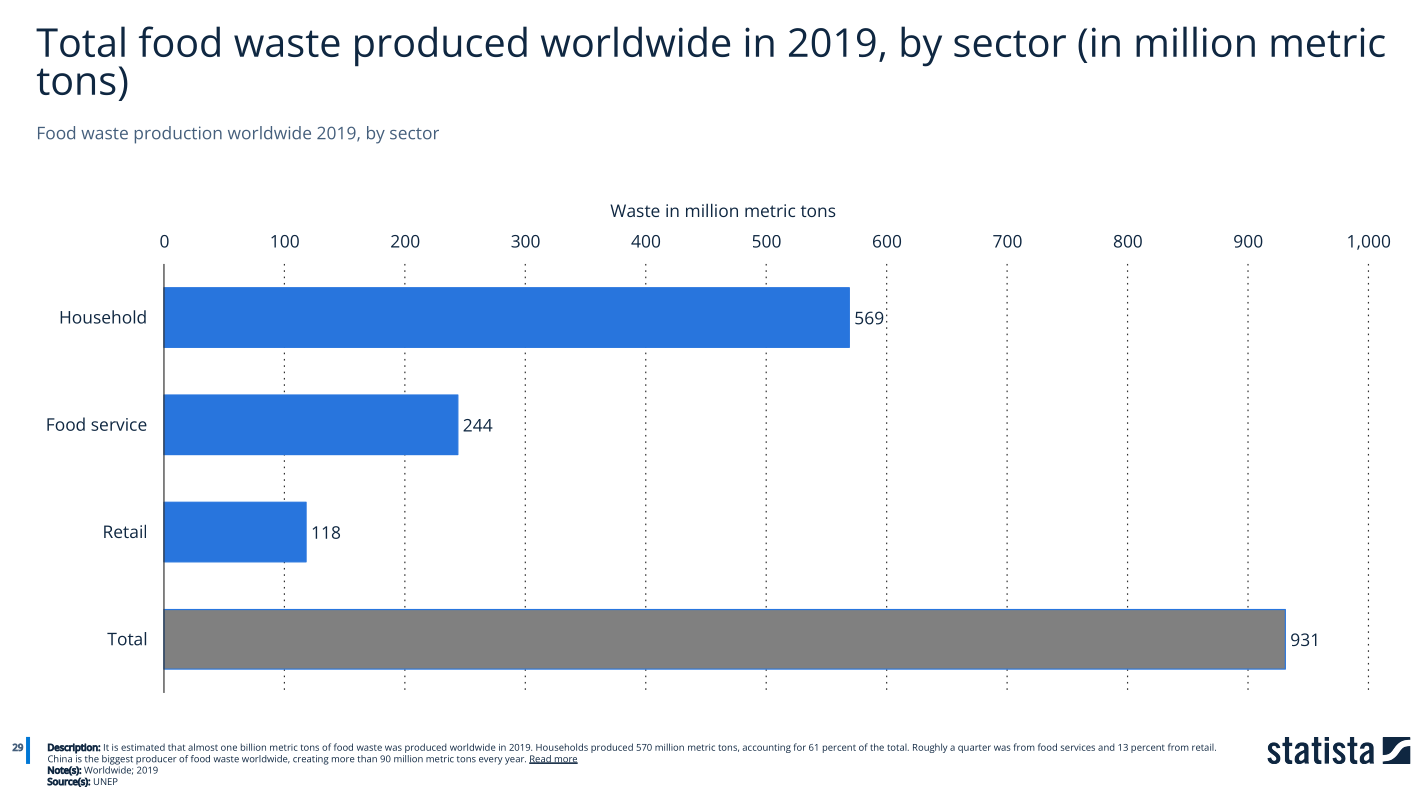
\includegraphics[width=.9\linewidth]{../plots/statistics/statistic_food_waste_by_sector_2019.png}
\caption{\label{fig:orge19f8e8}Παγκόσμια παραγωγή υπολειμμάτων τροφών ανά τομέα}
\end{figure}

Η Ελλάδα είναι η χώρα με την δεύτερη μεγαλύτερη παραγωγή οικιακών υπολειμμάτων τροφών κατά κεφαλήν παγκοσμίως (142 κιλά/άτομο ετησίως) (“Statista - The Statistics Portal” n.d.) . Η παραγωγή υπολειμμάτων τροφών, ειδικά στον τομέα της κατανάλωσης, όπου βρίσκονται τα οικιακά υπολείμματα, καθώς και αυτά της εστίασης, είναι πολύ συχνά αναπόφευχτη. Οπότε, παρόλο που με πιο σωστές πρακτικές θα μπορούσαν να παράγονται λιγότερα υπολείμματα, η ανάπτυξη τεχνολογιών αξιοποίησης των υπολειμμάτων αυτών είναι πάρα πολύ σημαντικές. Οι τεχνολογίες αυτές θα πρέπει να είναι εύκολα εφαρμόσιμες και οικονομικές και η κλιμάκωση τους να είναι εφικτή.

Γενικά, η αγορά της διαχείρισης αποβλήτων είναι αρκετά μεγάλη (υπολογίζεται περίπου στα 1293 δις δολλάρια ετησίως από μία μελέτη του 2022), ενώ προβλέψεις λένε πως θα φτάσει τα 2000 δις μέχρι το 2030 και τα οργανικά απόβλητα, ως ένα πολύ σημαντικό ποσοστό των αστικών αποβλήτων (περίπου \(40-45 \%\)) είναι μία από τις βασικές περιοχές ενδιαφέροντος της αγοράς αυτής (“Statista - The Statistics Portal” n.d.) . Μία από τις βασικότερες τεχνολογίες που έχουν αναδειχθεί σε αυτήν την αγορά η οποία έχει δει ραγδαία αύξηση τα τελευταία χρόνια είναι η αναερόβια χώνευση. Η αναερόβια χώνευση χρησιμοποιεί οργανικά απόβλητα ως υπόστρωμα και με μία σειρά βιοχημικών διεργασιών, τα μετατρέπει σε πτητικά λιπαρά οξέα (VFAs) και τελικά μεθάνιο και διοξείδιο του άνθρακα (το μίγμα γνωστό ως βιοαέριο), το οποίο είναι ένας πολύ καλός ενεργειακός φορέας. Τα υπολείμματα τροφών είναι ένα πολύ καλό υπόστρωμα για αναερόβια χώνευση καθώς είναι πλούσια σε οργανικές ενώσεις αλλά και θρεπτικά στοιχεία και μπορούν να μετατραπούν πολύ αποτελεσματικά σε βιοαέριο. Στο \figurename\textasciitilde{} \ref{fig:org929c288} φαίνεται η παγκόσμια παραγωγή ενέργειας από βιοαέριο τα τελευταία 15 χρόνια (“Statista - The Statistics Portal” n.d.) .

\begin{figure}[htbp]
\centering
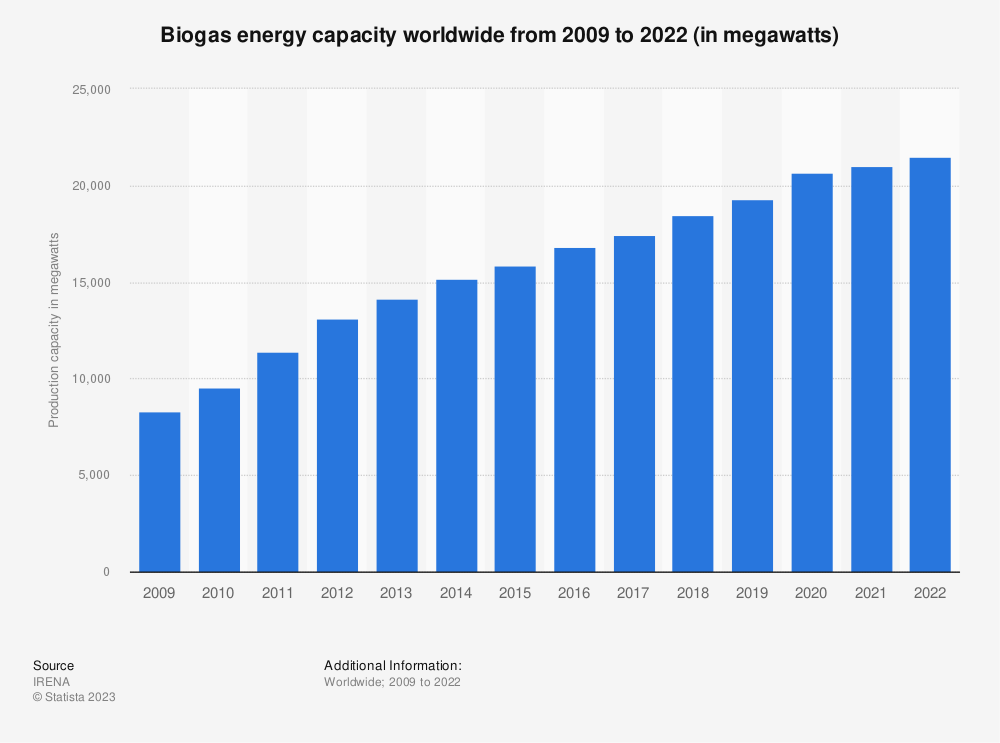
\includegraphics[width=.9\linewidth]{../plots/statistics/statistic_id1032922_global-biogas-energy-capacity-2009-2022.png}
\caption{\label{fig:org929c288}Παγκόσμια παραγωγή ενέργειας από βιοαέριο}
\end{figure}

Εκτός όμως από την αξιοποίηση του μεγάλου βιοχημικού δυναμικού των υπολειμμάτων αυτών, η αναερόβια χώνευση λύνει και άλλο ένα από τα σημαντικά προβλήματα του 21ου αιώνα, το οποίο είναι η ενέργεια. Αυτή τη στιγμή, πάνω από το \(80 \%\) της ενέργειας που καταναλώνεται παγκοσμίως βασίζεται σε μη ανανεώσιμες πηγές όπως το πετρέλαιο και το φυσικό αέριο. Οι ενεργειακές απαιτήσεις παγκοσμίως έχουν μία συνεχή αύξηση, ενώ οι πρώτες ύλες αυτές εξαλείφονται (“Statista - The Statistics Portal” n.d.) . Οπότε, τεχνολογίες παραγωγής ενέργειας από ανανεώσιμες πηγές, οι οποίες να έχουν το δυναμικό να αντικαταστήσουν τις πηγές αυτές θα γίνουν απαραίτητες τα επόμενα χρόνια. Οι περισσότερες τεχνολογίες ανανεώσιμης ενέργειας (πχ αιολική, ηλιακή ή υδροηλεκτρική ενέργεια) έχουν δυσκολία να φτάσουν τέτοια επίπεδα και για αυτό χρησιμοποιούνται επικουρικά σε μία κύρια πηγή ενέργειας (αυτή τη στιγμή, περίπου το \(30 \%\) της παγκόσμιας παραγωγής ηλεκτρισμού οφείλεται σε τέτοιες πηγές) (“Statista - The Statistics Portal” n.d.) . Τα υπολείμματα τροφών από την άλλη είναι άφθονα οπότε θεωρείται πως μία αποτελεσματική επεξεργασία θα μπορέσουν να καλύψουν ένα πολύ σημαντικό ποσοστό της παγκόσμιας ανάγκης σε ενέργεια.

Σκοπός της παρούσας μελέτης είναι η ανάπτυξη μίας μεθόδου επεξεργασίας των υπολειμμάτων τροφίμων, αρχικά, μέσω της βιοαποδόμησής τους με χρήση σκευασμάτων ενζύμων και μικροοργανισμών του εμπορίου, και στη συνέχεια, μέσω αναερόβιας χώνευσης για την παραγωγή βιοαερίου, η οποία θα αξιολογηθεί σε εργαστηριακή αλλά και πιλοτική κλίμακα.
\end{document}
